\section{Realisierung}
\subsection{Vorgehensweise}
Zu Beginn wurde ein Plan für das grobe Zusammenspiel der beteiligten Komponenten angefertigt. Hiermit wurde die Arbeit in mehrere Schritte und leicht abzugrenzende Komponenten unterteilt. Das Projekt ließ sich damit in Meilensteine aufteilen um strukturiert an das Projekt herangehen zu können.
\subsection{Analyse \& Konzeption}
Bei der Analyse der Anforderungen fallen die Realtime Aspekte auf. Sie sollen mithilfe von Websocketkommunikation und Push-Bases-Updates vom Server umgesetzt werden. Für einen modernen Look und ein intuitives Verhalten auf mobilen Geräten soll die Steuerung Drag and Drop unterstützen.
\subsubsection*{Architektur}
Einen groben Überblick über die spätere ``physikalische Ausprägung'' des Systems soll die Grafik~\ref{fig:architektur} geben.
\begin{figure}[h]
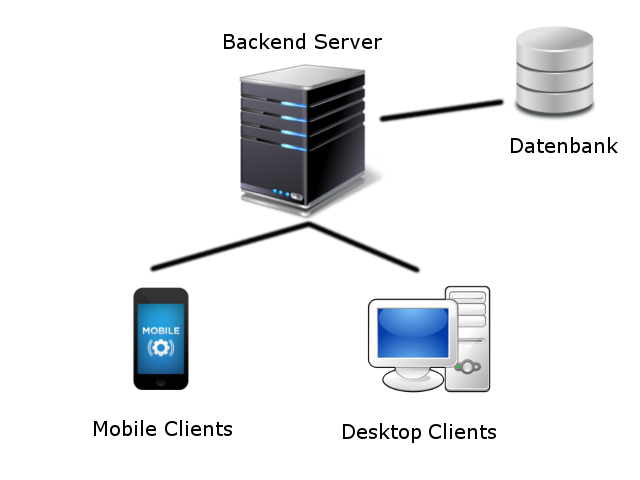
\includegraphics[scale=0.5]{img/Architektur.png}
\caption{Architektur Übersicht\label{fig:architektur}}
\end{figure}
Die Clients (Mobile / Desktop) kommunizieren über WebSockets mit dem Backend-Server. Dieser speichert und liest Daten aus einer Datenbank. Durch die WebSockets ist es dem Backend-Server möglich Änderungen am Datenmodell mittels Push-Benachrichtigungen an die Clients weiterzugeben.
\subsection{Implementierung}
\subsubsection{Browser-Frontend}
Die Implementierung des Browser-Frontends verwendet Technologien, die dem Reactive Pattern zuzuweisen sind.
React.js als UI-Framework von Facebook ist ein stark durch funktionale Ideen inspiriertes Framework. Das Browser Frontend ist modular aufgebaut. Die Kommunikation mittels WebSockets und das Verwalten des Applikationszustandes geschieht im in PureScript implementierten ``Frontend-Backend''. Diese sogenannte Engine nimmt im Unidirectional-Dataflow Modell die Rolle der ``Stores'' ein und erlaubt es das View-Layer beliebig auszutauschen.
\begin{figure}[h]
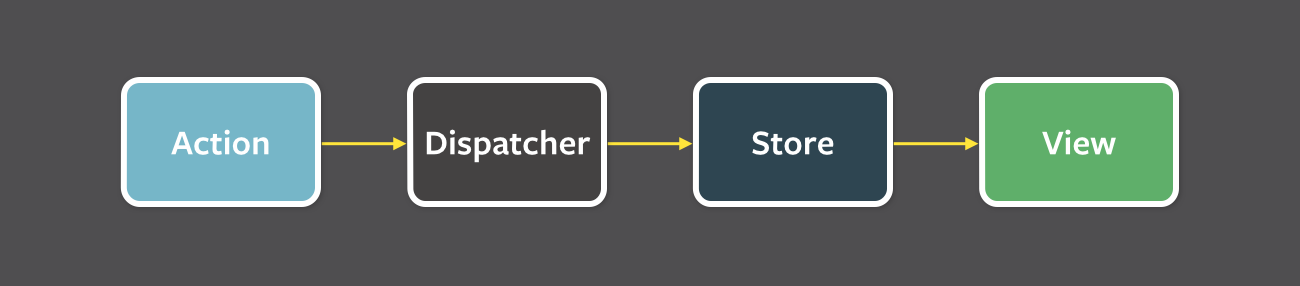
\includegraphics[scale=0.3]{img/Unidirectional.png}
\caption{Unidirectional Dataflow}
\end{figure}

Die Interaktionen des Benutzers mit dem View-Layer erzeugen dann wiederum Events, die als Streams an die Stores zurückfließen, wo sie interpretiert und verarbeitet werden. Das interpretieren der Events lässt sich dank des deklarativen Stils den PureScript erlaubt, leicht programmieren. Als Beispiel soll der Code dienen, der das Ziehen eines Topics auf das Grid beschreibt.


\begin{lstlisting}
  dragTopic = do
    Right t <- dragStart
    action <- dragOver
    lookup "dragEndTopic" `merge` lookup "dragEndGridTopic"
    return $ action t
\end{lstlisting}

\subsection{Test \& Abnahme}
\subsection{Projektablauf}
